\section{Kĩ thuật tăng nhiệt}
\label{sec:reheat}
Một trong những vấn đề mà nhiều thuật toán tìm kiếm lân cận gặp phải đó là bị mắc trong một nghiệm tối ưu địa phương. Điều này có nghĩa là, sau một khoảng thời gian tìm kiếm ta thấy rằng thuật toán không thể cải thiện nghiệm thêm nữa hoặc là qua rất nhiều bước lặp nữa mới tìm được một nghiệm tốt hơn. Có nhiều yếu tố ảnh hưởng đến hiện tượng này. Ví dụ, đối với ALNS, số lượng yêu cầu bỏ đi quá lớn hoặc quá nhỏ khiến cho các thuật toán chèn không tìm được vị trí tốt để thêm lại yêu cầu (khi mà các tuyến đã chật chội sau một khoảng thời gian chạy). Ngoài ra, tiêu chí chấp nhận nghiệm cũng ảnh hưởng rất nhiều. Đối với mô phỏng luyện kim, càng về sau chúng ta chỉ chấp nhận những nghiệm tốt hơn nghiệm tốt nhất đã biết hoặc là chấp nhận một nghiệm tệ hơn với giá trị chênh lệch rất nhỏ do tham số "nhiệt độ" của mô phỏng luyện kim đã nhỏ đi đáng kể sau thời gian chạy dài. Để khắc phục hiện tượng này, ta có thể sử dụng kĩ thuật tăng nhiệt (\textit{reheat}) để tăng "nhiệt độ" của mô phỏng luyện kim lên một giá trị nào đó trong những giai đoạn nhất định (Salwani và các cộng sự (2011) \cite{salwani2011re}). 

Có một vài cách tăng nhiệt khác nhau ví dụ như tăng nhiệt khi sau một số vòng lặp mà thuật toán không cải thiện được nghiệm hoặc tăng nhiệt sau một số vòng lặp nhất định (cố định). Trong quá trình thực nghiệm cho luận văn này, cách thứ hai được sử dụng. Tăng nhiệt không cần thiết phải sử dụng với các cấu hình quá nhỏ hoặc thời gian chạy ngắn vì nó cũng không tìm ra nghiệm tốt hơn (đáng kể) khi không sử dụng. 

\begin{figure}[H] % places figure environment here   
  \centering % Centers Graphic
  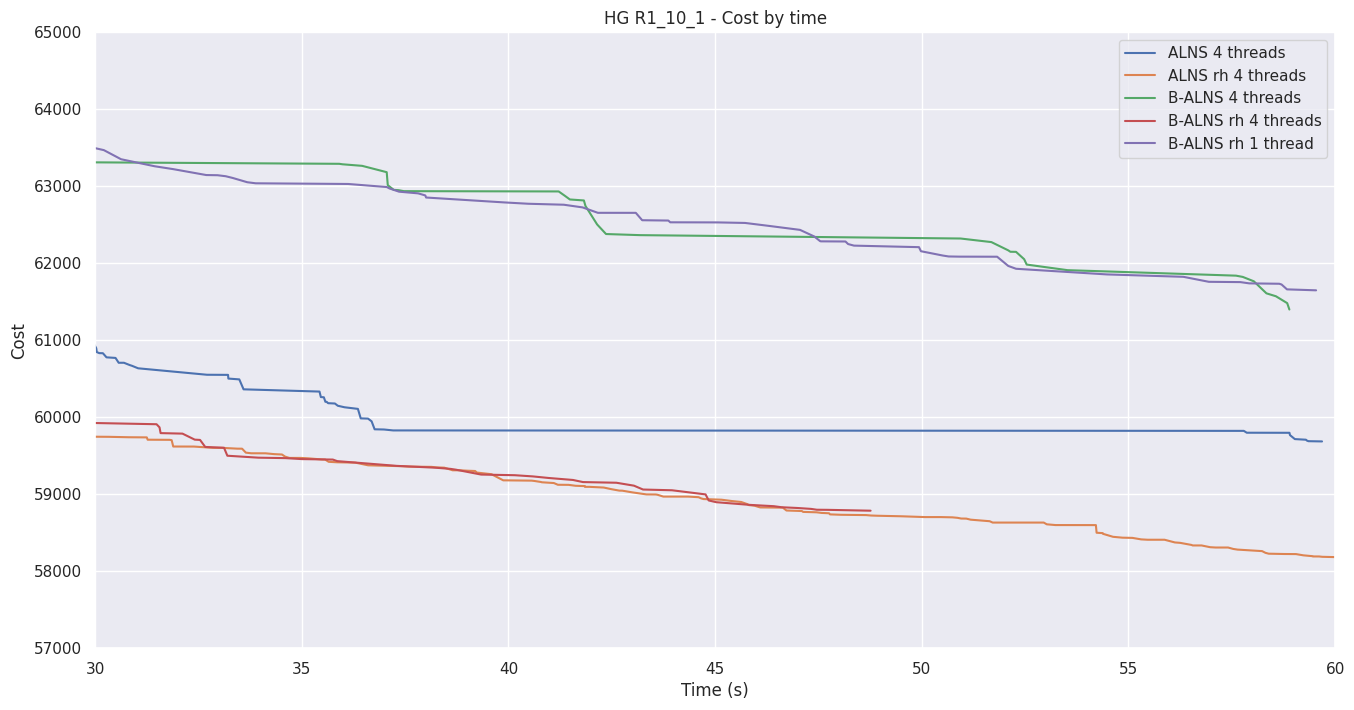
\includegraphics[width=1\textwidth]{figures/cost_time_R1_10_1_rh.png} 
  % \includesvg[scale=1]{figures/core-object}
  \caption{Hàm mục tiêu theo thời gian với một số cách chạy khác nhau cho cấu hình \code{R1\_10\_1} (\textit{rh biểu thị cho các thuật toán áp dụng kĩ thuật tăng nhiệt}).} 
  \label{fig:reheat1}
\end{figure}

Một điểm thú vị là kĩ thuật tăng nhiệt giúp cho B-ALNS "thoát" được nghiệm tối ưu địa phương khi đã trải qua thời gian chạy dài. Không những vậy tăng nhiệt giúp các thuật toán tìm được nghiệm tốt hơn khi so với không dùng tăng nhiệt.